\chapter{Laboratorio: Programación Flip-flops, Contadores, Drivers.}


\section{Objetivos}
Este es un laboratorio introductorio que busca:
\begin{itemize}
	{\small
	 \item  Programar en ARDUINO el comportamiento de los Flip-Flop J-K, T, D activador por flanco positivo y el Biestable Set-Reset.
	 \item  Estudiar que los Flip-Flop usan reloj para sincronizar los cambios pero los biestables son asincrónicos.
	 \item  Programar en ARDUINO el comportamiento de un Contador ascendente decendente para el control de un parqueo.
	 \item  Programar un driver para un motor unipolar y bipolar con Arduino.
 }
\end{itemize} 


\section{Equipos y materiales}
Para este laboratorio de necesitaran:
\begin{itemize}
	{\small \item 1 Arduino UNO o equivalente: MEGA o ESP32.
	\item 1 Multímetro.
	\item 10 Resistencias de 270 o 330 $\Omega$.
	\item 5 Resistencias de 1k$\Omega$.
	\item 10 interruptores pulsadores.
	\item 1 Protoboard.
	\item 1 display de 16 x 2 segmentos.
	\item 1 motor a pasos bipolar.
	\item 1 chip L293D con dos puentes H para motor bipolar.
	\item 1 motor a pasos unipolar. 
	\item 1 driver 28BYJ-48 para motor unipolar con driver  ULN2003.
	\item 1 Computadora portátil.}
\end{itemize}

\section{Marco de referencia}

 Los sistemas secuenciales tienen la característica que sus salidas en cualquier momento determinado son funciones tanto de las entradas externas en ese momento como de la secuencia de salidas pasadas. Esto quiere decir que esas salidas son memorizadas para usarlas como entrada en el siguiente análisis. El análisis de las entradas y memorias se ejecuta en los flanco positivos o negativos de una señal de control o reloj.
 
 Los dispositivos encargados de memorizar solo son capaces de almacenar información binaria, es decir un cero o uno lógico. Estos elementos de memoria son llamados cerrojos y bi-estables (\textit{latches} y \textit{flip-flops} ) , y la diferencia principal entre estos dos tipos de elementos es que los primeros son asincrónicos, es decir no dependen de una señal de reloj, y los segundos (\textit{flip-flops}) si dependen de un reloj externo. 

Existen varios tipos de cerrojos y bi-estables, pero para efectos del laboratorio se estudiarán el cerrojo Set-Reset, y los bi-estables J-K, D, T. El cerrojo S-R tienen las siguientes ecuaciones características:

\begin{eqnarray}
\label{lab3:Ec1}
Q=S+Q\bar{R} \\ \label{lab3:Ec2}
Q=(S+Q)\bar{R}
\end{eqnarray}
donde $S$ es la entrada que pone un uno lógico en la salida $Q$, por otro lado la entrada $R$ restablece la salida $Q$. La ecuación \eqref{lab3:Ec1} da prioridad a la entrada set, mientras que la ecuación \eqref{lab3:Ec2} da prioridad a la entrada reset. El Cuadro \ref{tab:SR} muestra el comportamiento esperado del cerrojo S-R, si el S-R es con prioridad al Set la X vale un uno lógico, y si es prioridad al reset la X vale un cero lógico. 

\begin{table}
	\centering
	\caption{Tabla de verdad del cerrojo S-R.}
	\label{tab:SR}
	\begin{tabular}{|c|c|c|c|}
		
		\hline 
		$S$ 	& $R$  & $Q+$  & $\bar{Q}+$  \\
		\hline 
		0	& 0 &	$Q$	&	$Q$		\\ 
		
		0	& 1&	0	&	1	\\ 
		
		1	& 0 &	1	&	0	\\ 
			
		1	& 1 &	X	&	X	\\ 	
		\hline 
	\end{tabular} 
\end{table} 

Los bi-estables J-K poseen poseen tres entradas: J, K y el reloj Clk. La ecuación característica esta defina por \eqref{lab3:Ec4}, mientras que la tabla de verdad se presenta en el Cuadro \ref{tab:JK}. 

\begin{eqnarray}
	\label{lab3:Ec4}
%%	Q=J\bar{Q}+Q\bar{K} \\ \label{lab3:Ec5}
	Q=(J\bar{Q}+Q\bar{K})\cdot\uparrow CLK
\end{eqnarray}


\begin{table}
	\centering
	\caption{Tabla de verdad del Latch J-K.}
	\label{tab:JK}
	\begin{tabular}{|c|c|c|c|c|}
		
		\hline 
		$J$ 	& $K$  & $CLK$  &  Q+ &$\bar{Q}+$ \\
		\hline 
		X	& X &	X	&	$Q$	&  $\bar{Q}$	\\ 
		0	& 0 &	$\uparrow$	&	$Q$	&  $\bar{Q}$	\\ 
		0	& 1&	$\uparrow$	&	0  &   1	  \\ 
		1	& 0 &   $\uparrow$	&	1  &   0	\\ 	
		1	& 1 &	$\uparrow$	&	$\bar{Q}$   &  $Q$	 \\ 	
		\hline 
	\end{tabular} 
\end{table} 

Por otra parte los bi-estable tipo de D y T son casos particulares del bi-estable J-K y sus ecuaciones características estan definas por \eqref{lab3:Ec6} y \eqref{lab3:Ec7}. 

\begin{eqnarray}
\label{lab3:Ec6}
Q=D\cdot\uparrow CLK \\ \label{lab3:Ec7}
Q=(T\bar{Q}+Q\bar{T})\cdot\uparrow CLK
\end{eqnarray}


\subsection{Implementación de Cerrojos y Biestables}

La implementación de cerrojos y bi-estables dependen de como se llamen las funciones características de los elementos de memoria. Para los cerrojos se llaman en la rutina principal y los biestables se llaman dentro de un rutina de interrupción por hardware.

El \textit{latch Set-Reset} con prioridad al reset es una función que se implementa en la sección de funciones de la siguiente forma,

		 \begin{lstlisting}[language=Arduino,numbers=none, showstringspaces=false]
		bool RS(bool S,bool R,bool Q){
			return  (S||Q)&&!R;
		}
		\end{lstlisting} donde $S$ y $R$ son entradas digitales y $Q$ es una variable global del tipo booleano. Al no de pender de una señal de reloj, esta función se llama dentro del rutina principal \textbf{loop()}.

Por otra parte, los \textit{flip-flop} funcionan si existe un flanco positivo o negativo de reloj, para emular este comportamiento se usa  la interrupción por \textit{hardware}, pin 2 o 3  en un Arduino UNO. La interrupción por hardawre se habilita dentro de la sección \textbf{setup()}, con el comando \href{https://reference.arduino.cc/reference/en/language/functions/external-interrupts/attachinterrupt/}{ \textbf{attachInterrupt()}}.

	\begin{lstlisting}[language=Arduino,numbers=none, showstringspaces=false]

void setup(){
// Initializa los pines:
	{
		//Linas de código
	}	
	/* Habilita la Rutina de Interrpcion por Hardware (RIH) en
	cada flanco positivo que se detecta en PIN #2 */
	
	attachInterrupt(digitalPinToInterrupt(2), RIH, RISING);
}
\end{lstlisting}

La rutina de interrupción detiene la rutina principal \textbf{loop()} y ejecuta una rutina definida por el usuario llamada en este caso RIH. Esta rutina no posee parametros de entrada, ni de salida. Dentro de la rutina  RIH si se puede llamar a otras funciones programadas, por ejemplo se llama la función del bi-estable J-K definida en la sección de funciones. 


		\begin{lstlisting}[language=Arduino,numbers=none, showstringspaces=false]
		
		bool JK(bool J, bool K, bool Q){
			return (J&&!Q)||(!K&&Q);
		}
		\end{lstlisting}

\subsection{Contadores y Secuenciadores}


El diseño digital de contadores, secuenciadores como por ejemplo la lógica de control parar motores a pasos (\textit{drivers}) se simplifica con un lenguaje de alto nivel como C/C++, por lo tanto no es necesario implementar como si fuera un diseño digital, en cambio usaremos funciones y estructuras de control. Por ejemplo un contador ascendente/descendente de 0-20 se puede programar de forma similar a función \textbf{Contador()}.
\begin{lstlisting}[language=Arduino,numbers=none, showstringspaces=false]
int Contador (bool Sube, bool Baja, int Valor){
	if (Sube && (Valor <20)){
		Valor++;
	}
	if(Baja && (Valor >0)){
		Valor--;
	}
	return Valor;
}
\end{lstlisting}
 
De manera similar un secuenciador de cuatro etapas que genere la secuencia $\{1100_{2}, 0110_{2}, 0011_{2}, 1001_{2}\}$ o su equivalente en decimal    $\{12,6,3,9\}$, puede servir para controlar los relays o transistores de un \href{https://es.wikipedia.org/wiki/Motor_paso_a_paso}{motor a pasos}. La función para controlar un motor a pasos unipolar es similar a la siguiente:


\begin{lstlisting}[language=Arduino,numbers=none, showstringspaces=false]

byte Driver(int Paso){
	byte output = 0;
	if(Paso==1){
		output=0b00001100; 
	}
	if(Paso==2){
		output=0b00000110;
	}
	if(Paso==3){
		output=0b00000011;
	}
	if(Paso>=4){
		output=0b00001001;
	}
	return output;
}
\end{lstlisting} donde el parámetro de entrada (Paso), es el resultado dado por un una función que cuenta entre {1-4}. Si el resultado del la función \textbf{Driver()} se desea imprimir a los pines digitales, esto se realiza con la función \href{https://www.arduino.cc/reference/en/language/functions/bits-and-bytes/bitread/}{\textbf{bitRead()}} .
  
\section{Metodología}

Este laboratorio tiene una duración de 4 lecciones, repartidas en dos semanas. Los estudiantes deben mostrar durante las clases programadas las tres actividades propuestas. Deben recabar fotografías y resultados de los equipos de medición para elaborar las evidencias. Las evidencias se subirán al TecDigital la semana siguiente finalizadas las actividades.

\section{Práctica en Clase}

\subsection{Actividad 1}

Programe un Arduino Uno con el comportamiento de un Latch Set-Reset prioridad al set, y los flip-flops J-K, T, D.  Por el pin 2 entra una señal de reloj con frecuencia ajustable entre 5Hz y 1kHz. El Pin 3  se conecta a una botonera y representar\'a las  S, J, D y T.  El pin 4 se conecta a otra botonera y se  reserva para la entrada R y K. La salida del cerrojo S-R se muestra mediante a un LED conectado al PIN 4. El Pin 5 se conecta a otro LED y será la salida del Bi-estable J-K. Los pines 6 y 7, son las salidas de los flip-flops T y D y también se conectan a LEDs. Imprima los resultados en el puerto serial, ajuste la velocidad del puerto con valores de: \{ 9600, 14400, 19200, 28800, 38400, 57600\}bps según la frecuencia del reloj.
 
\subsubsection{Conteste las preguntas}

¿Es el comportamiento programado es idéntico a la tablas de verdad teóricas o existen diferencias? Explique.
¿Cual es la diferencia práctica entre un S-R y un J-K? ¿Cual responde más rápido?,
¿Que pasa si el reloj posee una frecuencia de 1KHz, son las respuestas distintas o iguales? Explique. 
¿Como son las gráficas obtenidas si los datos se gráficas en Excel?

\subsection{Actividad 2}

Se desea automatizar un paqueo automotriz que posee exactamente 20 campos disponibles. El parqueo tiene una entrada y una salida como se aprecia en la Figura \ref{fig:parqueo}. 

Tanto la entrada como la salida posee sensores de proximidad (usted usará 2 botones pulsadores para emular  esto). Además el Arduino controlará las 2 agujas de acceso (2 LEDs). Cuando un automóvil ingrese al parqueo, se abrirá la aguja (LED) si y solo si hay cupo disponible, sino el LCD parpadeará el número cero. Si se abre la aguja usted debe mostrar en la pantalla del LCD cuando cupos quedan disponibles. Por otra parte cuando sale un carro también se incrementa en uno los campos disponibles y se muestra en el LCD.

Cuando se abre cualquier aguja, el LED que lo representa, debe permanecer encendido por 5 segundos y luego se apagará.

El Display posee una estructura de 16 x 2 caracteres, en el primer reglón colocarán el contador de cupos disponibles como se aprecia en la figura \ref{fig:dislay}. En el segundo reglón aparecerá durante el tiempo que LED  este encendido las palabras ENTRADA $>$ o SALIDA $<$  respectivamente. Recuerde que un vehículo puede ingresar mientras otro esta saliendo y viceversa.

\begin{figure}
	\centering
	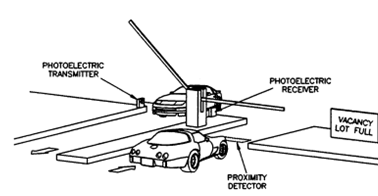
\includegraphics[width=0.7\linewidth]{fig/Parqueo.png}
	\caption{Entrada y salida del parqueo.}
	\label{fig:parqueo}
\end{figure}

\begin{figure}
	\centering
	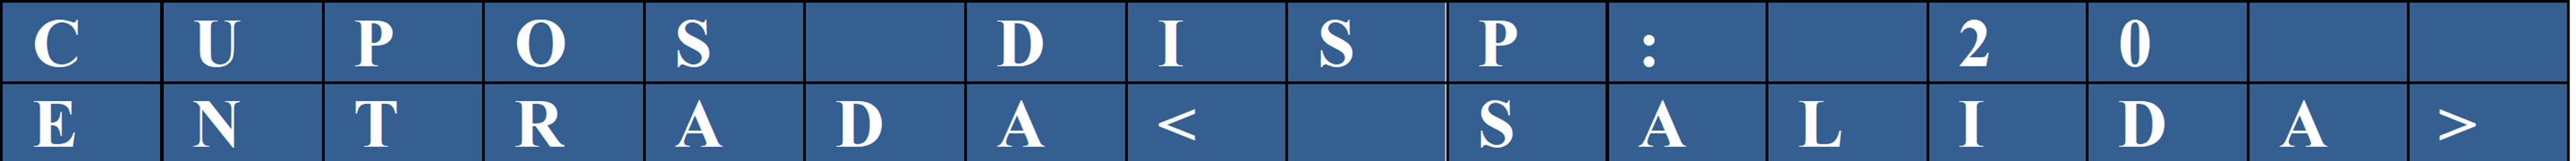
\includegraphics[width=0.7\linewidth]{fig/Dislay.png}
	\caption{Display de 16 x 2 caracteres.}
	\label{fig:dislay}
\end{figure}

Para realizar esta actividad debe estudiar los siguiente:
 Estudiar la \href{https://docs.arduino.cc/software/ide-v1/tutorials/installing-libraries#.Uyd116h5PRk}{instalación de librerías} en Arduino. En Arduino existen mas de cuatro mil librerías que pueden ser consultadas en este \href{https://www.arduino.cc/reference/en/libraries/}{enlace}.
 Estudiar el uso de un display 16x2 caracteres usando la librería \href{http://arduino.cc/en/Tutorial/LiquidCrystalDisplay#.UyPQYfl5OSo }{\textbf{LiquidCrystal.h}}.
 Estudiar la librerías \href{https://github.com/sstaub/Timer}{\textbf{Timer.h }}, \href{https://github.com/kiryanenko/SimpleTimer}{\textbf{SimpleTimer.h}} para la generación de pulsos controlados.
 
\subsubsection{Conteste las preguntas:}

¿Que pasa si ambos botones, entrada y salida, se presionan de forma simultanea?
¿Puede realizar un experimento completo donde se muestre como se llena y vacía el parqueo y exportar los resultados al puerto serial?

\subsection{Actividad 3}

Realice un programa en Arduino que controle dos motores a pasos, con un botón conectado al Pin 1 los dos motores arrancan o paran. Si se arranca los motores, en pantalla se mostrará la palabra RUN, y el sentido de giro  de giro derecho ($>>$).
\begin{figure}[h]
	\centering
	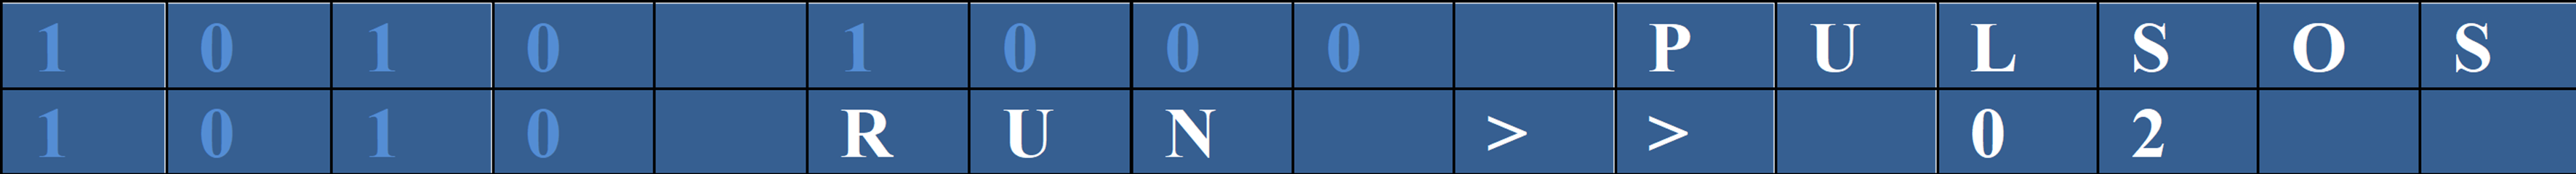
\includegraphics[width=0.7\linewidth]{fig/Fig3.png}
	\caption{Display 16X2 caracteres.}
	\label{fig:fig3}
\end{figure}
Si se presiona el nuevamene Pin 1 (pare), los motores se detienen indicando la palabra STOP en el Display de cristal liquido (LCD).
\begin{figure}[H]
	\centering
	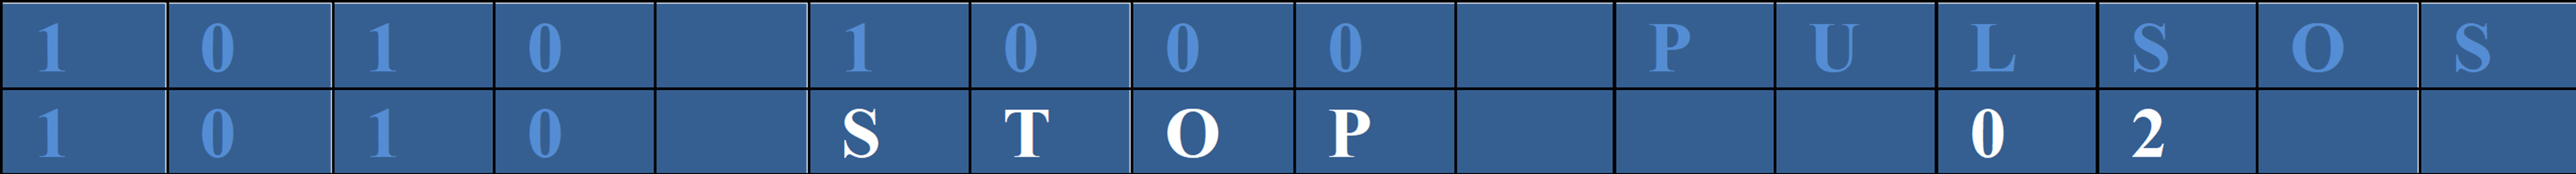
\includegraphics[width=0.7\linewidth]{fig/Fig4.png}
	\caption{Información mostrada en Display cuando se presiona el boton de parada.}
	\label{fig:fig4}
\end{figure}

Si presiona el botón conectado al PIN (3) en la pantalla los dos motores cambiaran de sentido de giro, y en pantalla aparecerá ($<<$). Si se presiona nuevamente el botón conectado al Pin (2), los motores cambiaran de sentido nuevamente y en pantalla aparecerá ($>>$).

Si se presionan botones UP o DOWN (Pines 4 o 5) la velocidad de pulsos por segundo se incrementará ($\uparrow$) o se excrementará ($\downarrow$) de uno en uno, desde 2 p/sec hasta 40p/sec. En pantalla se montará las siguientes flechas.
\begin{figure}[H]
	\centering
	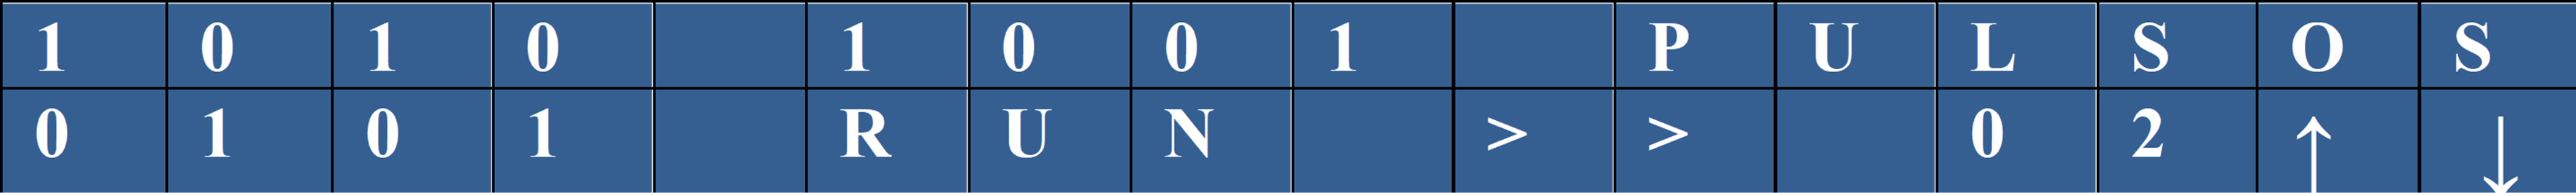
\includegraphics[width=0.7\linewidth]{Imagenes/Fig5}
	\caption{Flechas mostradas en Display cuando se modifican los pulsos. }
	\label{fig:fig5}
\end{figure}
Los motores unipolares se controlan con las señales S1, S2, S3, S4 que se muestran en el Display. Los motores Bipolar necesitan dos puentes H y cada puente tendrá las señales de control Q1, Q2, Q3, Q4.  Las señales de control Sx y Qx tendrán valores de 1 o 0 únicamente.

\begin{figure}[H]
	\centering
	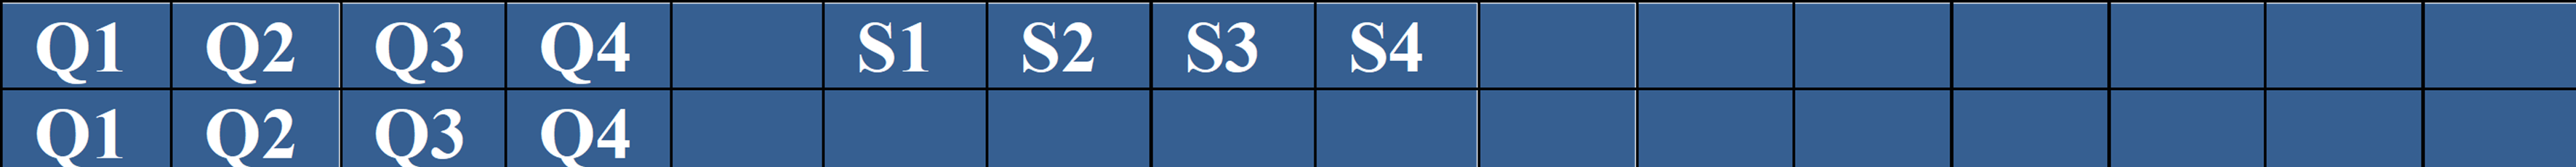
\includegraphics[width=0.7\linewidth]{Imagenes/Fig6}
	\caption{Señales de control para los motores.}
	\label{fig:fig6}
\end{figure}

El circuito de potencia de un puente H se aprecia en la figura \ref{fig:puenteh}.
\begin{figure}[H]
	\centering
	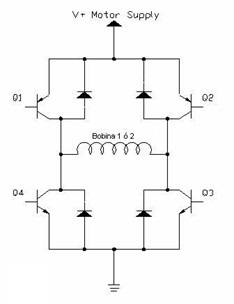
\includegraphics[width=0.4\linewidth]{Imagenes/PuenteH}
	\caption{Puente H para un motor Bipolar.}
	\label{fig:puenteh}
\end{figure}

Conecte un motor Unipolar o bipolar con el circuito de potencia al Arduino. Utilize el circuito de potencia adecuado según su motor. Ponga en el Eje cinta para ver el sentido de jiro.

\subsubsection{Conteste las preguntas:} 

¿Puede mostrar las tablas de excitación generadas por el arduino para controlar los motores?
¿Son estas tablas similares a la teóricas?